\tikzstyle{s} = [rectangle, rounded corners, minimum width=2cm, text width=3cm, minimum height=1cm, text centered, draw=black]
\tikzstyle{arrow} = [thick,->,>=stealth]
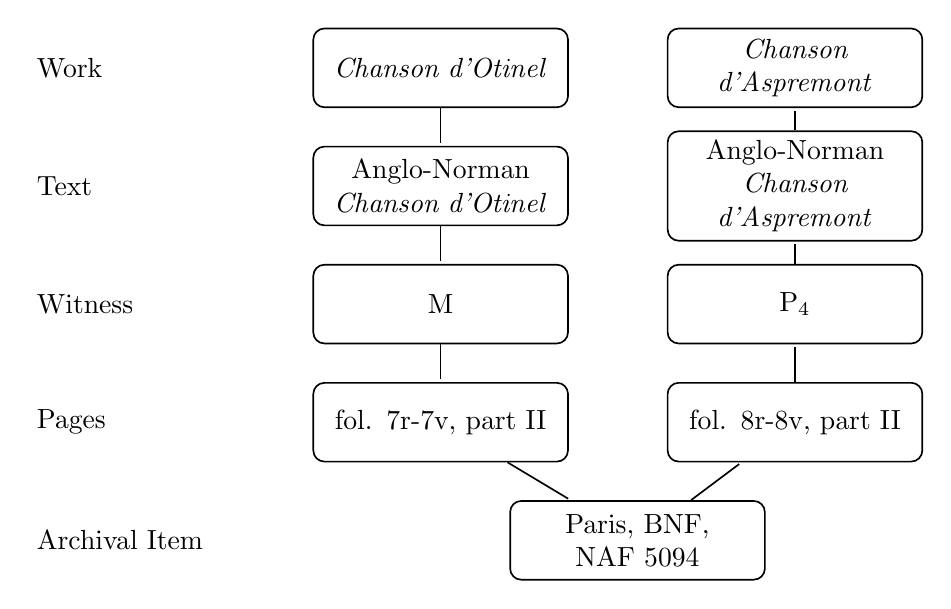
\begin{tikzpicture}[-,shorten >=1pt,auto,node distance=1.5cm,semithick]
\tikzstyle{every state}=[fill=red,draw=none,text=white]


\node[s] (WorkOtinel) {\textit{Chanson d'Otinel}};
\node[s] (WorkAspremont) [right of=WorkOtinel, xshift=3cm] {\textit{Chanson d'Aspremont}};
\node [left=2cm, text width=3cm] at (WorkOtinel) {Work};

\node[s] (ExpressionOtinel) [below of=WorkOtinel] {Anglo-Norman \textit{Chanson d'Otinel}};
\node[s] (ExpressionAspremont) [below of=WorkAspremont] {Anglo-Norman \textit{Chanson d'Aspremont}};
\node [left=2cm, text width=3cm] at (ExpressionOtinel) {Text};

\node[s] (ManifestationOtinel) [below of=ExpressionOtinel] {M};
\node[s] (ManifestationAspremontC) [below of=ExpressionAspremont] {P\textsubscript{4}};
% \node[s] (ManifestationAspremontP) [below of=ExpressionAspremont, xshift=2cm] {P\textsubscript{4}};
\node [left=2cm, text width=3cm] at (ManifestationOtinel) {Witness};

\node[s] (PagesOtinel) [below of=ManifestationOtinel] {fol. 7r-7v, part II};
\node[s] (PagesAspremontC) [below of=ManifestationAspremontC] {fol. 8r-8v, part II};
% \node[s] (PagesAspremontP) [below of=ManifestationAspremontP] {fol. 1r-2a};
\node [left=2cm, text width=3cm] at (PagesOtinel) {Pages};

\node[s] (ItemBNF) [below of=PagesOtinel, xshift=2.5cm] {Paris, BNF, NAF 5094};
% \node[s] (ItemCF) [below of=PagesAspremontP, xshift=-2cm] {Clermont-Ferrand, Arch. Dép., I F2};
\node[left=4.5cm, text width=3cm] at (ItemBNF) {Archival Item};

\path[every node/.style={font=\sffamily\small}]
    (WorkOtinel) edge node [right] {} (ExpressionOtinel)
    (ExpressionOtinel) edge node [right] {} (ManifestationOtinel)
    (ManifestationOtinel) edge node [right] {} (PagesOtinel)
    (PagesOtinel) edge node [right] {} (ItemBNF)
    (ItemBNF) edge node [right] {} (PagesAspremontC)
    (PagesAspremontC) edge node [right] {} (ManifestationAspremontC)
    (ManifestationAspremontC) edge node [right] {} (ExpressionAspremont)
    (ExpressionAspremont) edge node [right] {} (WorkAspremont)
    ;

% \path[every node/.style={font=\sffamily\small}]
%     (ExpressionAspremont) edge node [right] {} (ManifestationAspremontP)
%     (ManifestationAspremontP) edge node [right] {} (PagesAspremontP)
%     (PagesAspremontP) edge node [right] {} (ItemCF)
% ;

\end{tikzpicture}